\documentclass{article}

\addtolength{\oddsidemargin}{-.875in}
\addtolength{\evensidemargin}{-.875in}
\addtolength{\textwidth}{1.75in}
\addtolength{\topmargin}{-.875in}
\addtolength{\textheight}{1.75in}

\usepackage{amssymb, amsthm, amstext, amsxtra, amsmath, amsfonts, amscd }
\usepackage{graphicx, epsfig, apacite, dirtytalk, fancyhdr}
\usepackage{comment, color, cleveref, listings, wrapfig}
 

\pagestyle{fancy}
\fancyhf{}
\fancyhead[L]{Bayesian Data Analysis}
\fancyhead[R]{ \leftmark}
\fancyfoot[C]{\thepage}

\definecolor{dkgreen}{rgb}{0,0.6,0}
\definecolor{gray}{rgb}{0.5,0.5,0.5}
\definecolor{mauve}{rgb}{0.58,0,0.82}
\definecolor{backcolour}{rgb}{0.95,0.95,0.92}


\lstdefinestyle{R}{frame=tb, backgroundcolor=\color{backcolour}, 
				   language=R, 
				   aboveskip=3mm, belowskip=3mm, 
				   showstringspaces=false,
				   columns=flexible, numbers=none, tabsize=3,
				   keywordstyle=\color{blue}, 
				   numberstyle=\tiny\color{gray}, 
				   commentstyle=\color{dkgreen},
				   stringstyle=\color{mauve}, 
				   breaklines=true, 
				   breakatwhitespace=true}
\lstset{style=R}

\def\E{\mathbb{E}}
\def\pr{\mathbb{P}}
\renewcommand\baselinestretch{1.5}

\DeclareMathOperator{\sign}{sign}
\DeclareMathOperator{\supp}{supp}
\DeclareMathOperator{\Cov}{Cov}
\DeclareMathOperator{\Var}{Var}
\DeclareMathOperator{\corr}{corr}

\author{Salvador Garcia, s1655274}
\date{April 14th 2017}
\title{Report 2: Variance models for protein expression with missing data.}

\begin{document}

\maketitle

\section{Description of the problem} 

Concentration of 460 proteins was measured for each of 9 rats using images of 2D gels. Sensitivity of the equipment resulted in concentration values less than 5 to be treated as missing. The aim is to create an appropriate model for modelling variability of the concentration of proteins and of the missing data.

Let $X_{gr}$ be the observed concentration of protein $g$ in rat $r$, $g = 1; ... ; 460$ and $r = 1; ... ; 9$. It is known that the (unobserved) true concentration is different for different proteins however not much is known about their variability. A reasonable assumption is that their variability is similar or the same. Typically, logarithm of the concentration $X_{gr}$ is assumed to have a normal distribution:
 $Y_{gr} = \log{X_{gr}},$

 $$Y_{gr} | \mu_g \sigma_g^2 \sim N(\mu_g, \sigma_g^2)$$


\section{Modelling the variance}
\subsection*{Non-informative prior for $\mu_g$}
For the prior of $\mu_g$ I am going to use a normal prior with high variance $N(0, 1000)$ (As suggested in the lectures). Remembering, if we want to model the effect independently in each protein, we would like to use a vague prior.

\begin{figure}[ht!]
\centering
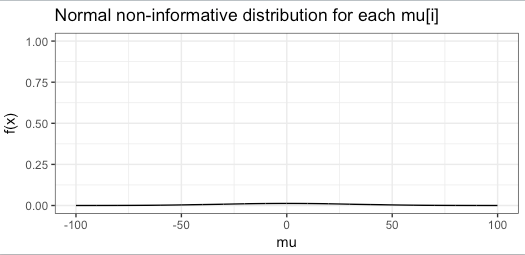
\includegraphics[width=12cm]{figures/00_prior1.png}
\end{figure}

\subsection*{ Bayesian models for the variance $\sigma_g^2$}

Three different models will be used for the variance. The first assumes equal variance for all the proteins $\sigma_g^2 = \sigma^2$ with a non-informative prior for $\sigma^2$ (In the code the prior was for $\tau$). The second and third are a hierarchical model for protein specific variance considering a log-normal and a gamma family each one.

\subsubsection*{ $\cdot\cdot\cdot\cdot\cdot$ Equal variance for all proteins $\sigma_g^2 = \sigma^2$ (model 1) $\cdot\cdot\cdot\cdot\cdot$}

\textbf{Burning, thinning and number of iterations}
For the first model 12000 iterations were done with a burning of 1001. No thinning was necessary. The inits for the first chain in the model were as follows: each $\mu_i$ was set with a value of 0, and $\tau=1$. In the second chain each $\mu_i$ had the value of 7 of $\tau = 6$. 

\begin{table}[ht!]
\centering
\caption{Criterias for the model}
\begin{tabular}{|l|l|}
\hline
Criteria             & Value \\ \hline
Number of iterations & 12000 \\ \hline
Thinning             & 1    \\ \hline
Burning              & 1001  \\ \hline
Number of chains     & 2     \\ \hline
\end{tabular}
\end{table}

\textbf{Model convergence and DIC}

First, I will analyze the convergence of the parameters $\mu_i$. To do that, the traceplots of the last 200 iterations (although all history was analyzed), the plots of the autocorrelations and the plots of the bgr diagnosis are show for the first 16 parameters $\mu_i$ (there are 413):
\begin{figure}[ht!]
\centering
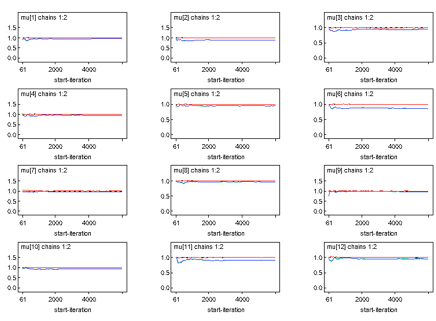
\includegraphics[width=13cm]{figures/model1_mu2.png}
\end{figure}


\begin{figure}[ht!]
\centering
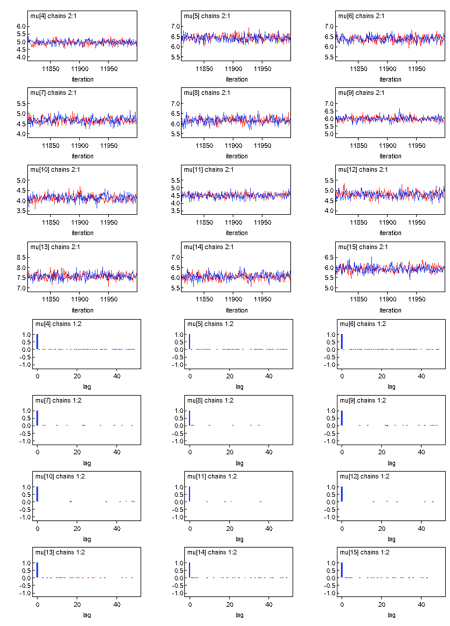
\includegraphics[width=12cm]{figures/model1_mu.png}
\end{figure}
 
These plots show that there are no problems with autocorrelation or convergence. The DIC for this model is the following:

\begin{figure}[ht!]
\centering
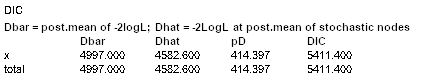
\includegraphics[width=12cm]{figures/model1_DIC.png}
\end{figure}
\newpage

The important part of the first section in the report is to model the variance. In this first model just one $\tau$ is assumed, and the prior for this parameter is a non-informative $Gamma(.01,.01)$ distribution. Now are presented the plots of the $\sigma$ and $\tau$ parameters. We can see that there is no problem of convergence or autocorrelation for these parameters.


\begin{figure}[ht!]
\centering
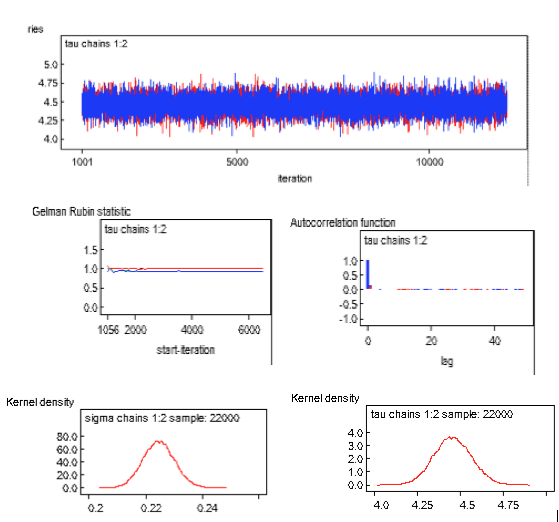
\includegraphics[width=14cm]{figures/model1_sigma.png}
\end{figure}

\begin{figure}[ht!]
\centering
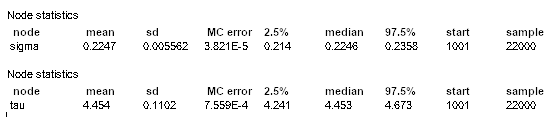
\includegraphics[width=14cm]{figures/model1_sigma2.png}
\end{figure}


\newpage


\subsubsection*{$\cdot\cdot\cdot\cdot\cdot$ Hierarchical models for protein specific variance $\sigma_g^2 | \theta \sim p(\theta)$ $\cdot\cdot\cdot\cdot\cdot$ }
For this subsection two families of distributions will be used to model. In the first a gamma distribution will be used as a prior for $\tau$ and in the second a lognormal distribution will be assumed for $\sigma$.

\underline{\textbf{Using a gamma distribution for the hyperparameters (model2)}}

\textbf{Burning, thinning and number of iterations}

For the second model, 12000 iterations were done with a burning of 1001. Again, no thinning was necessary. The inits for the first chain in the model were as follows: each $\mu_i$ was set with a value of 0, and each $\tau_i=1$. In the second chain each $\mu_i$ had the value of 6 of $\tau = 7$.  

\begin{table}[ht!]
\centering
\caption{Criterias for the model}
\begin{tabular}{|l|l|}
\hline
Criteria             & Value \\ \hline
Number of iterations & 12000 \\ \hline
Thinning             & 1    \\ \hline
Burning              & 1001  \\ \hline
Number of chains     & 2     \\ \hline
\end{tabular}
\end{table}

\textbf{Model convergence and DIC}

Now, I will analyze the convergence of the parameters $\mu_i$. To do that, the traceplots of the last 200 iterations (although all history was analyzed), the plots of the autocorrelations and the plots of the bgr diagnosis are show for the first 16 parameters $\mu_i$ (there are 413):

\begin{figure}[ht!]
\centering
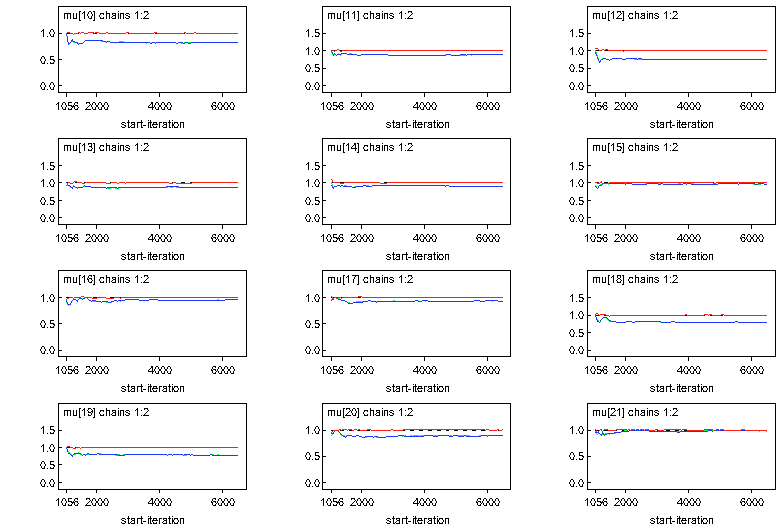
\includegraphics[width=14cm]{figures/model2_mu2.png}
\end{figure}


\begin{figure}[ht!]
\centering
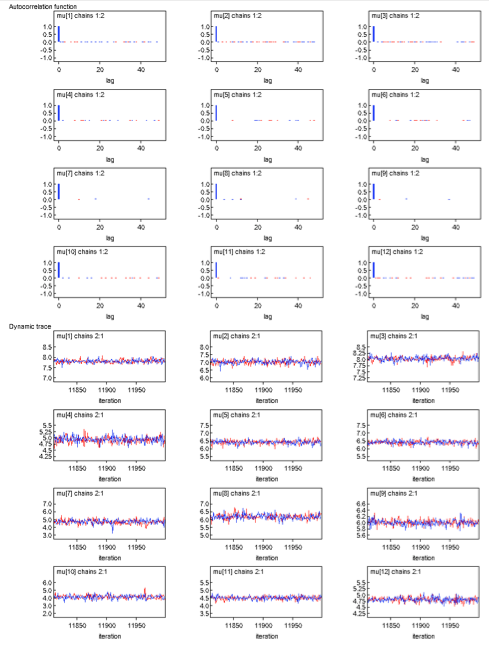
\includegraphics[width=14cm]{figures/model2_mu.png}
\end{figure}

\newpage
These plots show that there are no problems with autocorrelation or convergence. The DIC for this model is the following:

\begin{figure}[ht!]
\centering
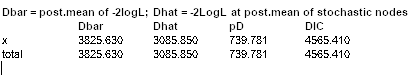
\includegraphics[width=12cm]{figures/model2_DIC.png}
\end{figure}


In this second model each row has a different $\tau_i$ parameter, and the prior for this parameters are a $Gamma(a,b)$ distribution, with $a, b$ hyperparameters with gamma non informative distribution. Now are presented the plots of the $\sigma$ and $\tau$ parameters. We can see that there is no problem of convergence or autocorrelation for these parameters:
\begin{figure}[ht!]
\centering
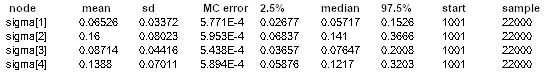
\includegraphics[width=12cm]{figures/model2_ultima.png}
\end{figure}
\begin{figure}[ht!]
\centering
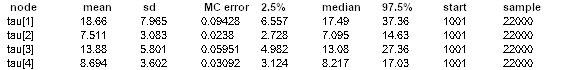
\includegraphics[width=12cm]{figures/model2_ultima2.png}
\end{figure}
\begin{figure}[ht!]
\centering
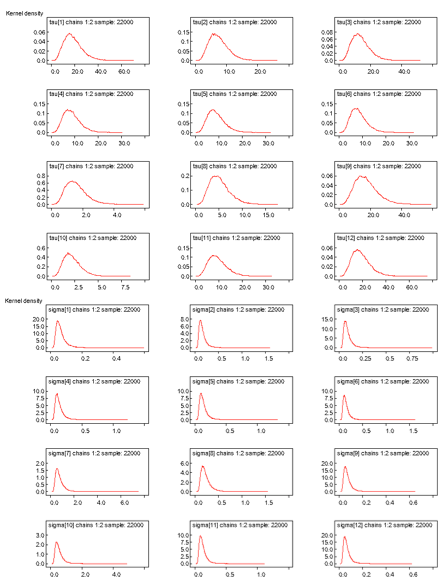
\includegraphics[width=12cm]{figures/model2_sigma.png}
\end{figure}

\newpage
\begin{figure}[ht!]
\centering
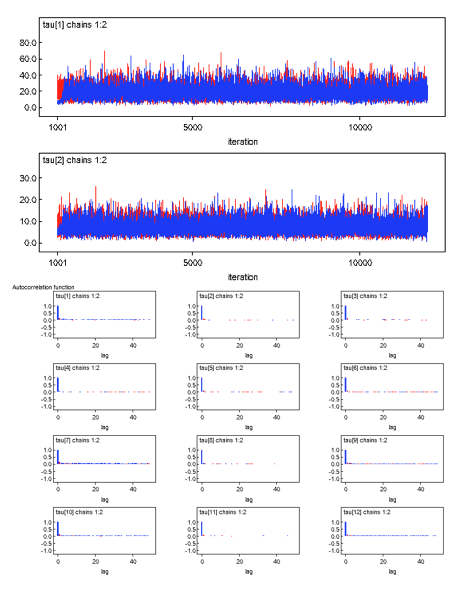
\includegraphics[width=11cm]{figures/model2_tau.png}
\end{figure}
\begin{figure}[ht!]
\centering
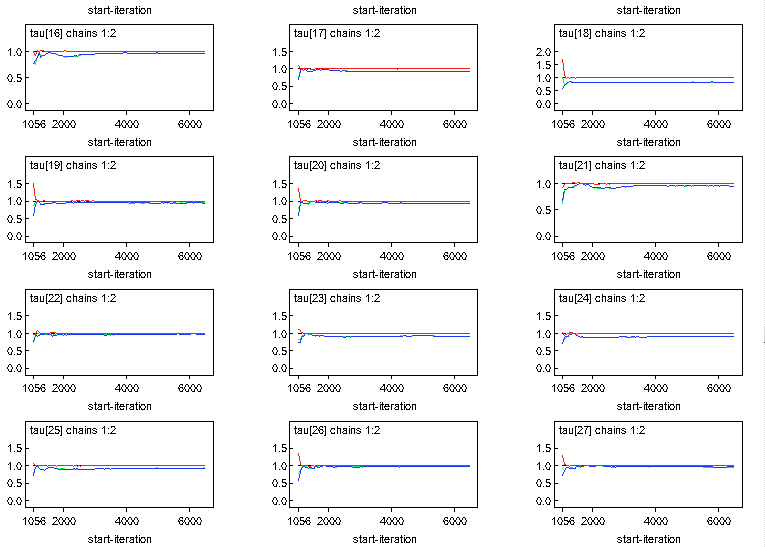
\includegraphics[width=11cm]{figures/model2_tau2.png}
\end{figure}


\newpage
\underline{\textbf{Using a lognormal distribution for the hyperparameters (model3)}}
For the third model, 15000 iterations were done with a burning of 2001. Again, no thinning was necessary. The inits for the first chain in the model were as follows: each $\mu_i$ was set with a value of 0, and each $\tau_i=1$. In the second chain each $\mu_i$ had the value of 6 of $\tau = 7$.  

\textbf{Burning, thinning and number of iterations}
\begin{table}[ht!]
\centering
\caption{Criterias for the model}
\begin{tabular}{|l|l|}
\hline
Criteria             & Value \\ \hline
Number of iterations & 6000 \\ \hline
Thinning             & 10    \\ \hline
Burning              & 501  \\ \hline
Number of chains     & 2     \\ \hline
\end{tabular}
\end{table}

\textbf{Model convergence and DIC}

Now, I will analyze the convergence of the parameters $\mu_i$. To do that, the traceplots of the last 200 iterations (although all history was analyzed), the plots of the autocorrelations and the plots of the bgr diagnosis are show for the first 16 parameters $\mu_i$ (there are 413):

\begin{figure}[ht!]
\centering
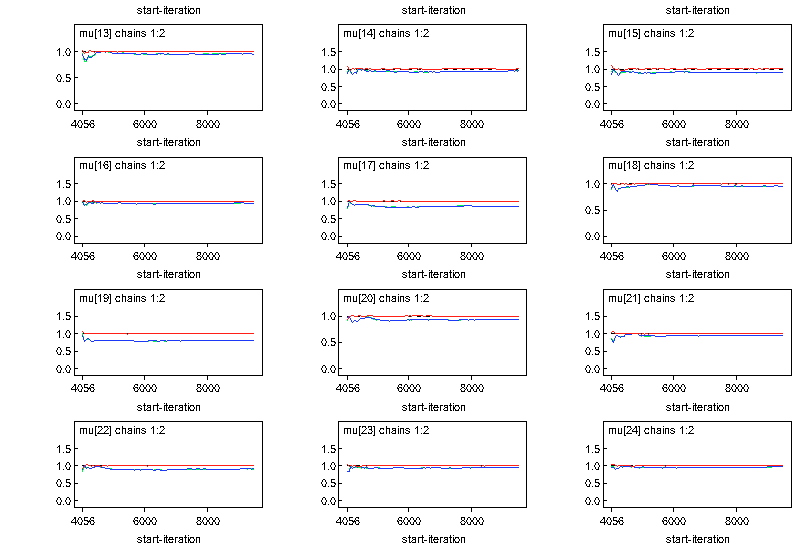
\includegraphics[width=14cm]{figures/model3_mu2.png}
\end{figure}

\begin{figure}[ht!]
\centering
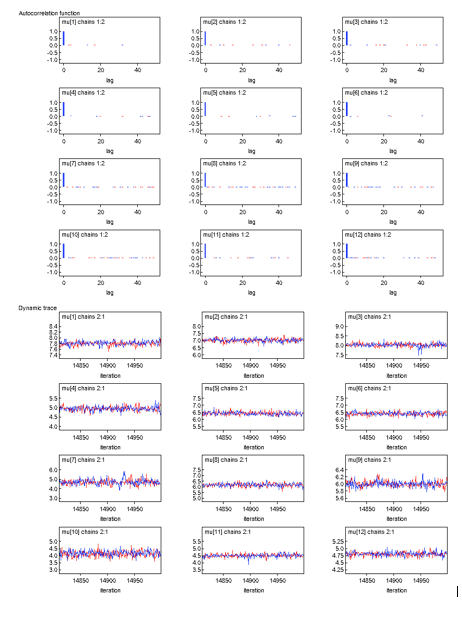
\includegraphics[width=14cm]{figures/model3_mu.png}
\end{figure}

\newpage
These plots show that there are no problems with autocorrelation or convergence. The DIC for this model is the following:

\begin{figure}[ht!]
\centering
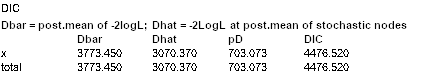
\includegraphics[width=12cm]{figures/model3_DIC.png}
\end{figure}
\newpage
Now, the parameters $\tau_i$ and $\sigma_i$ will be analized (just some of them):

\begin{figure}[ht!]
\centering
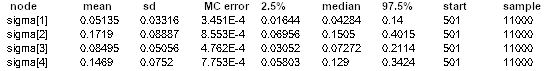
\includegraphics[width=12cm]{figures/model3_ultima.png}
\end{figure}

\begin{figure}[ht!]
\centering
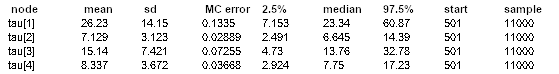
\includegraphics[width=12cm]{figures/model3_ultima2.png}
\end{figure}


\begin{figure}[ht!]
\centering
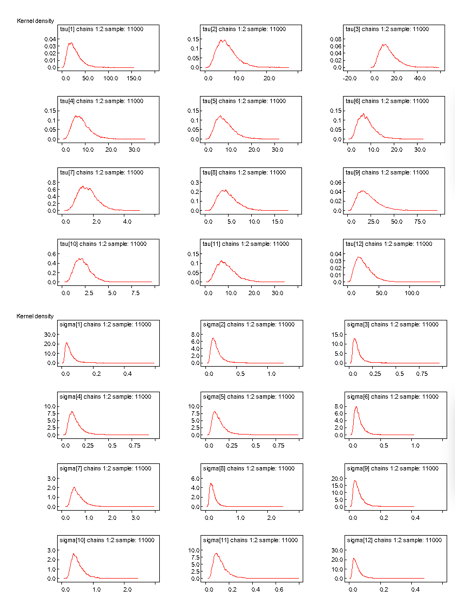
\includegraphics[width=12cm]{figures/model3_sigma.png}
\end{figure}


\begin{figure}[ht!]
\centering
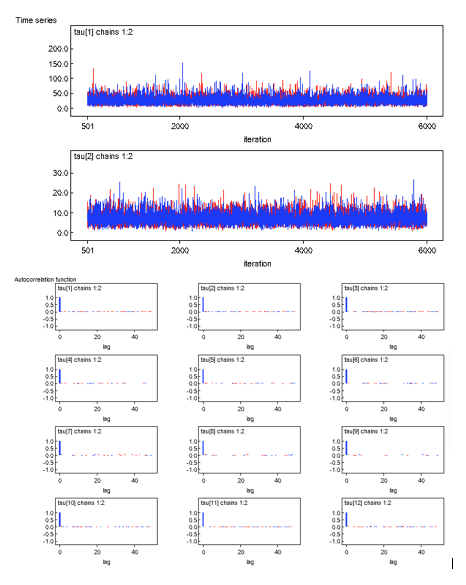
\includegraphics[width=12cm]{figures/model3_tau.png}
\end{figure}

\begin{figure}[ht!]
\centering
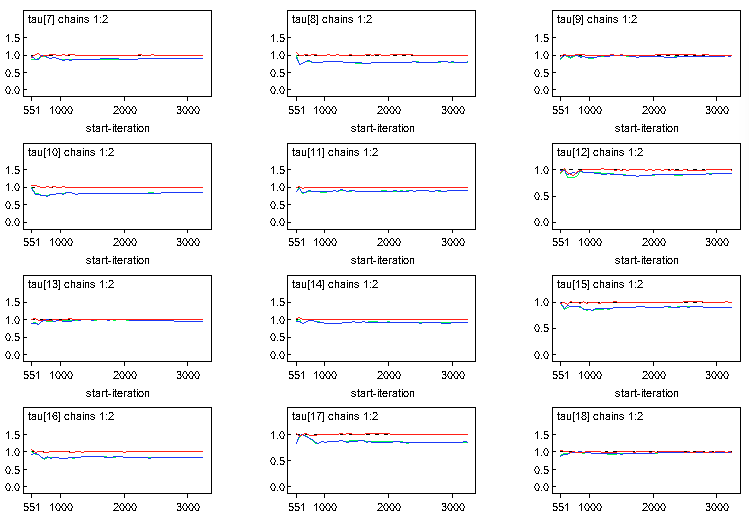
\includegraphics[width=10cm]{figures/model3_tau2.png}
\end{figure}


The following plots show no convergence problem. Also these does not show autocorrelation problems.

\newpage
\subsection*{Sensitivity to the prior of the parameters}
To check the sensitivity with the election of a gamma prior distribution for $\sigma_i$ or a lognormal, the mean and the 95\% confidence interval for $i = 1, ..., 413$ is shown below for both $\sigma$ and $\tau$ (the labels log($\sigma$) and log($\tau$) refers that the axis is in logarithm scale, not the values of $\sigma$ and $\tau$. This way, the values of tau are between $0-100$.)

\begin{figure}[ht!]
\centering
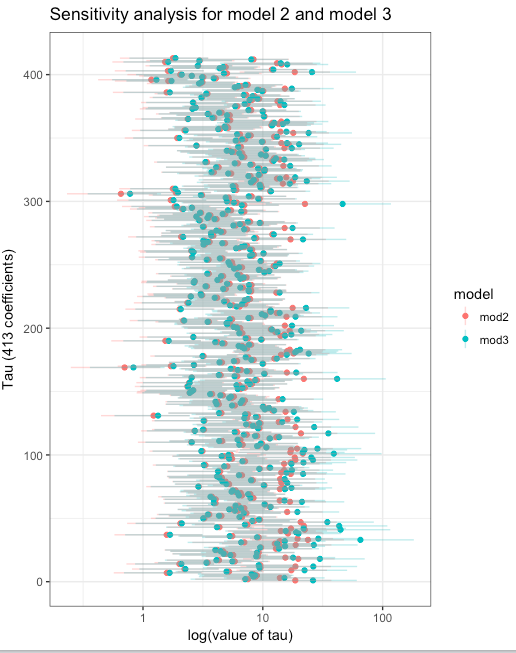
\includegraphics[width=15cm]{figures/model3_sensitivity.png}
\end{figure}

\begin{figure}[ht!]
\centering
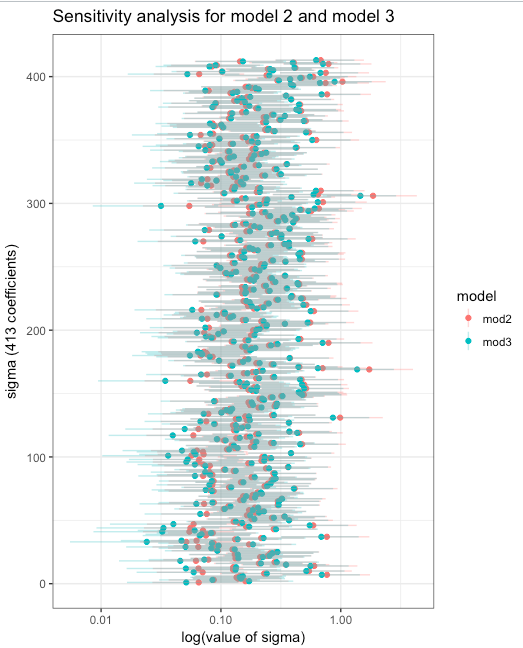
\includegraphics[width=15cm]{figures/model3_sensitivity2.png}
\end{figure}

\newpage
We can see that the distributions of $\sigma$ that have a mean close to 0 are a little bit different from model 2 to model 3 (and consequently the $\tau$ distribution is different). But, the values of the mean is different just by a small number, differing just in $.01$ or $.02$. Thus, we can assume that the selection of the prior has no important effect on the posterior distribution for $\tau$ and $\sigma$

\newpage
\subsection*{Best model: DIC, posterior predictive checks and mixed predictive checks $\theta$}

For the posterior predictive checks and the mixed predictive checks, I will follow the ideas presented in the slides:


\vspace{20mm}
\textbf{Posterior predictive checks} (From the slides) At each iteration $j = 1, ..., N$ of the MCMC sampler:
\begin{itemize}
	\item Generate $y_{grj}^{(pred)}$ from the full conditional for $y_{gr}^{(pred)}$
	\item Calculate  $S_{gj}^{2(pred)} = \frac{\sum_r (y_{grj}^{(pred)} - y_{g \cdot j}^{(pred)})^2}{9}$
	\item Calculate  $M_{gj} = I[S_{gj}^{2(pred)} \geq S_{gj}^{2(obs)}] $ 
\end{itemize}

The bayesian p-value for unit $g$ is $p_g= \frac{\sum_{j=1}^{413} M_{gj}}{413}$

\vspace{20mm}
\textbf{Mixed predictive checks} (From the slides) At each iteration $j = 1, ..., N$ of the MCMC sampler:
\begin{itemize}
	\item Generate $sigma_{gj}^{(pred)}$ from the full conditional for $\sigma_{g}^{(pred)}$
	\item Generate $y_{grj}^{(pred)}$ from the full conditional for $y_{gr}^{(pred)}$ (using the $\sigma_{gj}^{pred}$)
	\item Calculate  $S_{gj}^{2(pred)} = \frac{\sum_r (y_{grj}^{(pred)} - y_{g \cdot j}^{(pred)})^2}{9}$
	\item Calculate  $M_{gj} = I[S_{gj}^{2(pred)} \geq S_{gj}^{2(obs)}] $ 
\end{itemize}

The bayesian p-value for unit $g$ is $p_g= \frac{\sum_{j=1}^{413} M_{gj}}{413}$


\vspace{15mm}
According to the theory, the p-values follow an uniform distribution if model is \textit{true}.

\newpage

Now, for the first model just the posterior predictive checks will be made (no hyperpriors were used)

\underline{\textbf{First model}}
\begin{figure}[ht!]
\centering
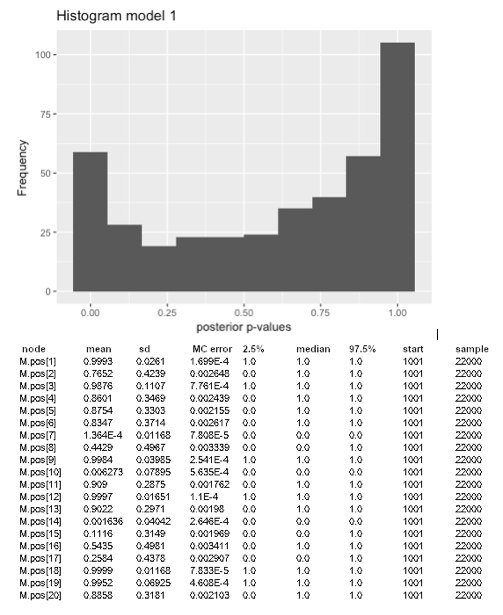
\includegraphics[width=14cm]{figures/model1_pospred.png}
\end{figure}

We can see that clearly, this does not follow an uniform distribution. For the second and third model, posterior predictive checks and mixed predictive checks will be made (as the methods in the lecture). As we can see, the plots related to the mixed predictive checks follows a more uniform distribution that the posterior predictive checks. Although is not perflectly uniform, the shape is very similar considering that we only have 413 elements.

\newpage
\underline{\textbf{Second model}}
\begin{figure}[ht!]
\centering
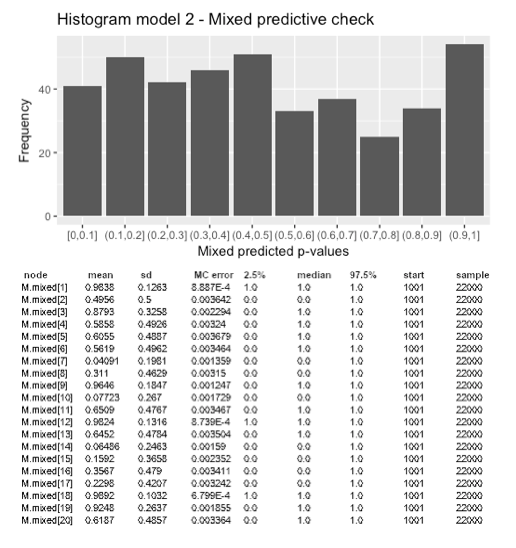
\includegraphics[width=10.1cm]{figures/model2_posmixpred.png}
\end{figure}

\begin{figure}[ht!]
\centering
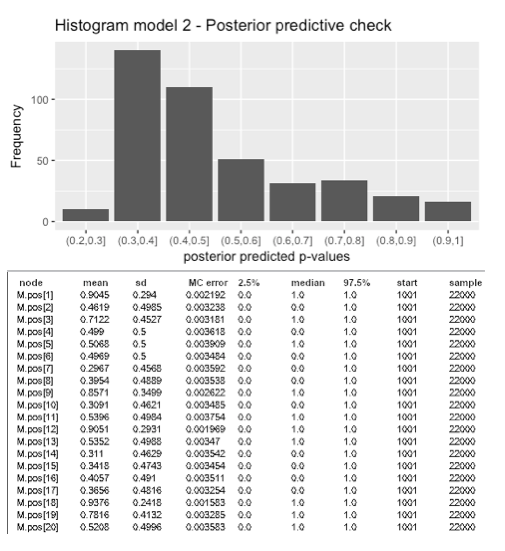
\includegraphics[width=10.1cm]{figures/model2_pospred.png}
\end{figure}

\newpage
\underline{\textbf{Third model}}

\begin{figure}[ht!]
\centering
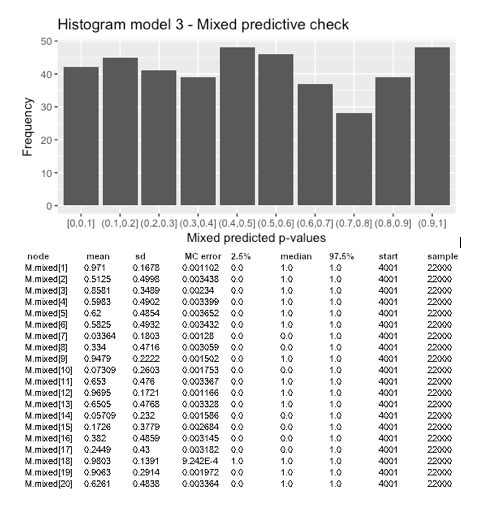
\includegraphics[width=10.4cm]{figures/model3_posmixpred.png}
\end{figure}

\begin{figure}[ht!]
\centering
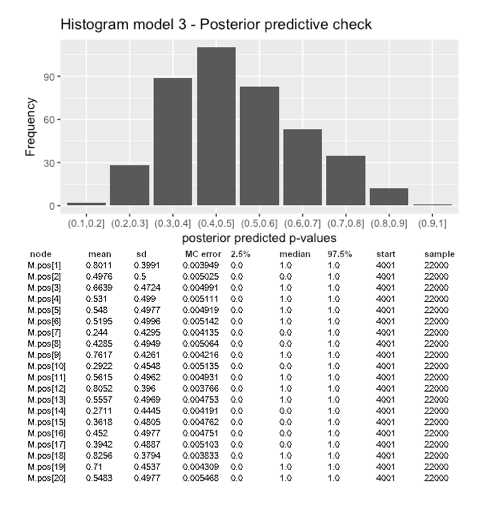
\includegraphics[width=10.4cm]{figures/model3_pospred.png}
\end{figure}

\newpage
Lastly, the DIC from the three models will be compared


\begin{table}[ht!]
\centering
\caption{DIC comparison}
\label{my-label}
\begin{tabular}{|l|l|}
\hline
Model                           & DIC \\ \hline
Model 1: Equal variance for all proteins & 5411.4   \\ \hline
Model 2: Hierarchical (gamma)	      & 4565.41   \\ \hline
Model 3: Hierarchical (log-normal)            & 4476.52   \\ \hline
\end{tabular}
\end{table}

From this table we can see that the best of the three models is the Hierarchical (log-normal).


\section{Missing values}
\subsection*{Missing at random assumption (MAR)}

At first sigth, the missing data sounds like a censored data problem \footnote{like the problem that arises when asking earning to people. People that earns too much money does not answer the question}, because the data that is less than 5 is missing, so the missigness depend on the value of the dependant variable. But, analyzing deeply the data, we can see that, for each protein \textbf{is not common} that values below 5 appear in the dataset (in the plot below is $\log(5)$ because $log(X_{gr}) \sim N(\mu_g, \sigma_g^2))$ :

\begin{figure}[ht!]
\centering
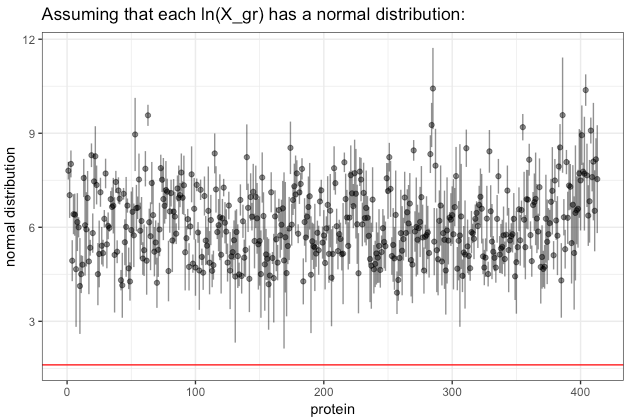
\includegraphics[width=12cm]{figures/missing.png}
\end{figure}

Now, the data does not look like a censored data problem. For me, it just seems as a method to eliminate noisy data that arises just because of external factors (or maybe just corrupted data). Thus, I will work with this problem with an \textit{ignorable missing data mechanism}. Another question that we have to ask is if the proteins with missing data are completely different than the proteins with no missing data (This to express the idea that the number of missign values is in function of the protein itself):

\newpage

\begin{figure}[ht!]
\centering
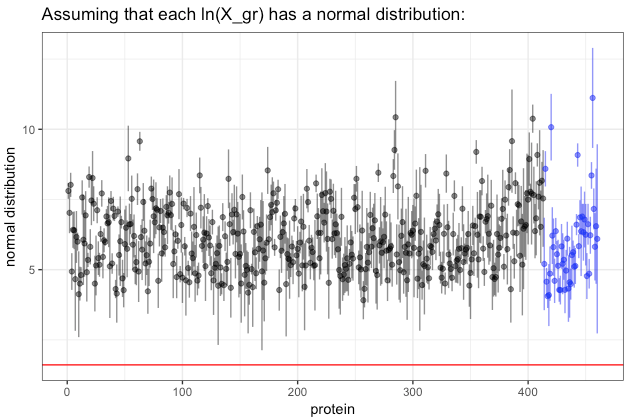
\includegraphics[width=12cm]{figures/missing2.png}
\end{figure}

In the above plot we can see that the empirical distribution of the data with missing values (in blue) is quite similar to the one that have complete data. There is no evidence to assume that the distributions are different (and in consequence a \textit{reason} to have missing values).

Some extra information that can be useful to analyze in order to know if the missing data has some estructure is the number of missing values per rat:

\begin{table}[ht!]
\centering
\caption{Number of missing values per rat}
\begin{tabular}{|l|l|l|l|}
\hline
Rat number & Missing values (MV) & (MV)/47 & (MV)/460 \\ \hline
1          & 0                   & 0 \%    & 0 \%     \\ \hline
2          & 6                   & 12.8 \% & 1.3\%    \\ \hline
3          & 25                  & 53.2 \% & 5.4\%    \\ \hline
4          & 5                   & 10.6\%  & 1.1\%    \\ \hline
5          & 8                   & 17.0\%  & 1.7\%    \\ \hline
6          & 12                  & 25.5\%  & 2.6\%    \\ \hline
7          & 4                   & 8.5\%   & 0.9\%    \\ \hline
8          & 11                  & 23.4\%  & 2.4\%    \\ \hline
9          & 9                   & 19.1\%  & 2.0\%    \\ \hline
\end{tabular}
\end{table}

The rat 3 has 25 missing values (that too much compared with the rat 1!). This show us that the missing values are not sufficiently at random, but we do not have sufficient evidence (it can be just by chance, the range are just from 0\% to 5.4\%). To make a conclussion about the relation rat number - number of missing values we would need more information or an explanation of this factor. 

As a conclusion and for the rest of this report, I will assume that the data is missing at random. 

\subsection*{Models for missing data}
For this section, the posterior distribution of the hyperparameters under the best model in section 1 is used as a prior distribution. I found impossible to use the exact posterior distribution found in section 1. As suggested, I will use the normal and gamma distributions that approximate these posteriors. (Although these do not completely especify the posterior distribution in the best model of section 1)

For each $\mu_i$ a Normal non-informative distribution was used $N(0, 1000)$. But, for the each $\tau_i$ a lognormal distribution was used with parameters $par_1, par_2$, with prior for $par_1 \sim N(\mu_{par_1}, \sigma_{par_1})$ and $par_2 \sim gamma(alpha_{par_2}, beta_{par_2})$. In the posterior summaries from section one, the mean and sd for each of these parameters are the next:

\begin{figure}[ht!]
\centering
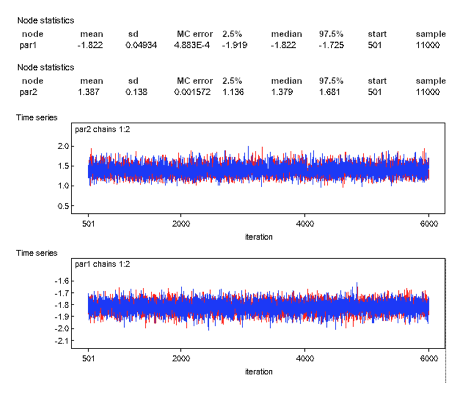
\includegraphics[width=16cm]{figures/model3_tau3_hyperpars.png}
\end{figure}

Then, $par_1$ can be approximated with a normal distribution $Normal(-1.822, 0.0024)$ (In terms of mean and variance). Equivalently, $par_2$ can be approximated with a lognormal distribution $lognormal(101.02, 72.83)$

Now, the analysis for missing data will be made in two ways. In the first, the missing data will be ignored (model 4). In the second, the missing data will be imputed (model 5). Because of the objective of the report, and to not make it excesivelly long, just the parameters $\sigma_i$ and $\tau_i$ will be analyzed

\newpage
\subsubsection*{Ignoring missing data (model 4) }

In this subsection, the used data file was $DataProteinsMissing.txt$. 11,000 iterations were made with a thinning of 10 and a burning of 1001. This datafile does not contains the missing values as NA. First, the autocorrelation and the density of the posterior distribution of the first 9 $\sigma_i$ will be analyzed:

\begin{figure}[ht!]
\centering
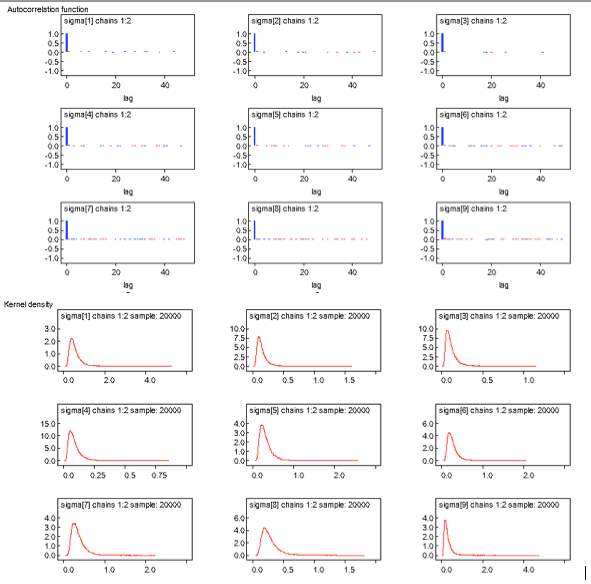
\includegraphics[width=16cm]{figures/model4_sigma.png}
\end{figure}


\newpage
Now, the bgr statistic and the chains will be analyzed. From the first we can see that the convergence looks good. For the second, we can observe that the chain looks good too.

\begin{figure}[ht!]
\centering
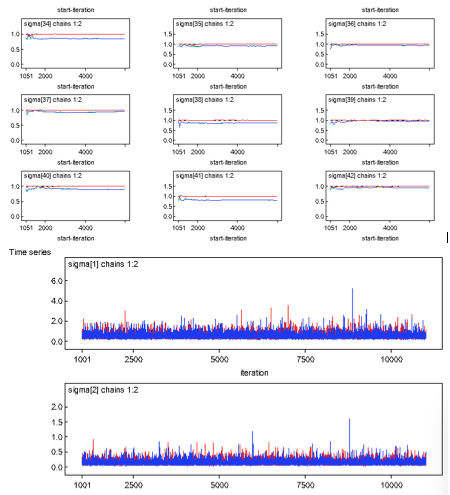
\includegraphics[width=14cm]{figures/model4_sigma2.png}
\end{figure}


\begin{figure}[ht!]
\centering
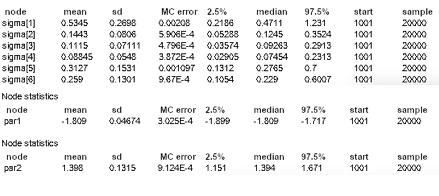
\includegraphics[width=12cm]{figures/model4_ultima.png}
\end{figure}

\newpage
\subsubsection*{Imputing values (model 5)}

In this subsection, the data file used was $DataProteinsMissingNA.txt$. 11,000 iterations were made with a thinning of 10 and a burning of 1001. This datafile contains the missing values as NA. First the autocorrelation and the density of the posterior distribution of the first 9 $\sigma_i$ will be analyzed:

\begin{figure}[ht!]
\centering
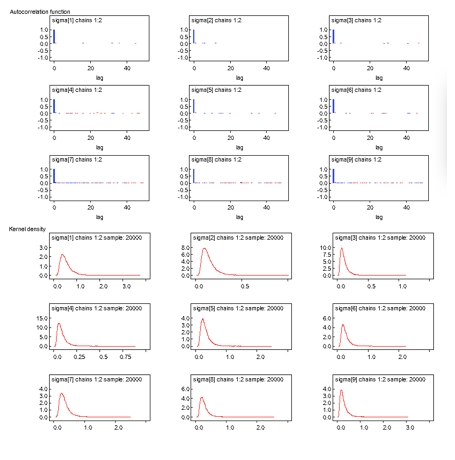
\includegraphics[width=16cm]{figures/model5_sigma.png}
\end{figure}


\newpage

Now, the bgr statistic and the chains will be analyzed. From the first we can see that the convergence looks good. For the second, we can observe that the chain looks good too.

\begin{figure}[ht!]
\centering
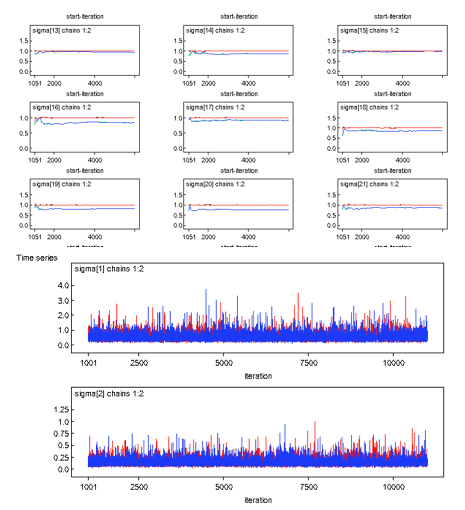
\includegraphics[width=14cm]{figures/model5_sigma2.png}
\end{figure}

\begin{figure}[ht!]
\centering
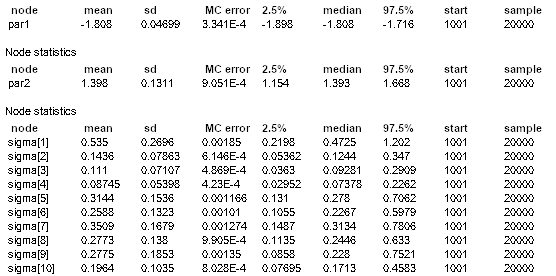
\includegraphics[width=12cm]{figures/model5_ultima.png}
\end{figure}

\newpage

\subsubsection*{Comparison model 4 and model 5}

To compare the model 4 and model 5, the distributions of each $\sigma_i$ are ploted together. In the next plot we can see how they look similar:

\begin{figure}[ht!]
\centering
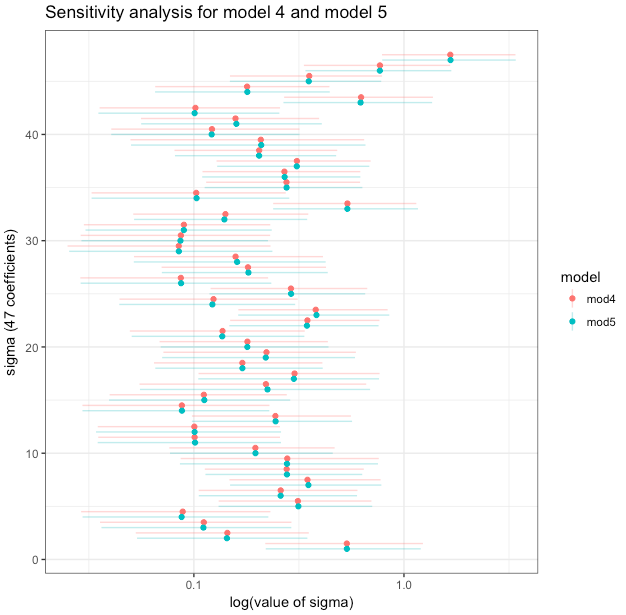
\includegraphics[width=12cm]{figures/model4_Sensitivity.png}
\end{figure}

As the slides of the course say \say{Results with missing data same as complete-case analysis here, since missing values are only in response, and mechanism is assumed ignorable}. In this example we have only missing values in response and we assumed ignorable the mechanism, so the distributions look almost the same.


\section{Conclusions}
From the first section of the report, the hierarchical model (with lognormal prior) is the best one. When trying to model the missing data I assume that the mechanism is ignorable (although I found some evidence that some rats have more missing values than others, but the difference was not very big. Also, we do not have information to assume that some "kind" of rats has more missing values, as the example in the slides of the fat rats). Some ideas to improve the models is to create variances for some groups of proteins (for example, make cluster of proteins and model just one variance for all of them).

\newpage
\section{Code for the models}

\subsection*{Model 1}
\begin{lstlisting}
model
{
	for( i in 1 : p ) {
		for( j in 1:n){
			x[i,j] <- log(y[i,j])
			x[i,j] ~ dnorm(mu[i], tau)
			
			# Posterior predictions
			pred.pos[i,j] ~ dnorm(mu[i], tau)
    	 }
	mean.orig[i]<- (x[i,1]+x[i,2]+x[i,3]+x[i,4]+x[i,5]+x[i,6]+x[i,7]+x[i,8]+x[i,9])/9
	s_2.orig[i]<-(pow(x[i,1]-mean.orig[i], 2)+pow(x[i,2]-mean.orig[i], 2)+pow(x[i,3]-mean.orig[i], 2)+pow(x[i,4]-mean.orig[i], 2)+pow(x[i,5]-mean.orig[i], 2)+pow(x[i,6]-mean.orig[i], 2)+pow(x[i,7]-mean.orig[i], 2)+pow(x[i,8]-mean.orig[i], 2)+pow(x[i,9]-mean.orig[i], 2))/9
	
	mean.pos[i] <- (pred.pos[i,1]+pred.pos[i,2]+pred.pos[i,3]+pred.pos[i,4]+pred.pos[i,5]+pred.pos[i,6]+pred.pos[i,7]+
	pred.pos[i,8]+pred.pos[i,9])/9
	
	s_2.pos[i] <- (pow(pred.pos[i,1]-mean.pos[i], 2)+pow(pred.pos[i,2]-mean.pos[i], 2)+pow(pred.pos[i,3]-mean.pos[i], 2)+pow(pred.pos[i,4]-mean.pos[i], 2)+pow(pred.pos[i,5]-mean.pos[i], 2)+pow(pred.pos[i,6]-mean.pos[i], 2)+pow(pred.pos[i,7]-mean.pos[i], 2)+pow(pred.pos[i,8]-mean.pos[i], 2)+pow(pred.pos[i,9]-mean.pos[i], 2))/9
	
	mu[i] ~ dnorm(0, .0001)
	M.pos[i] <- step(s_2.pos[i]-s_2.orig[i])
	diff[i] <- s_2.pos[i]-s_2.orig[i]
	}
	tau ~ dgamma(.01, .01)
	sigma <- 1/tau
	
}

\end{lstlisting}


\subsection*{Model 2}
\begin{lstlisting}
model
{
	for( i in 1 : p ) {
		for( j in 1:n){
			x[i,j] <- log(y[i,j])
			x[i,j] ~ dnorm(mu[i], tau[i])
			
			# Posterior predictions
			pred.pos[i,j] ~ dnorm(mu[i], tau[i])
			
			# Mixed predictions
			pred.mix[i,j] ~ dnorm(mu[i], tau.pred[i])
    	 }


	mean.orig[i]<- (x[i,1]+x[i,2]+x[i,3]+x[i,4]+x[i,5]+x[i,6]+x[i,7]+x[i,8]+x[i,9])/9
	s_2.orig[i]<-(pow(x[i,1]-mean.orig[i], 2)+pow(x[i,2]-mean.orig[i], 2)+pow(x[i,3]-mean.orig[i], 2)+pow(x[i,4]-mean.orig[i], 2)+pow(x[i,5]-mean.orig[i], 2)+pow(x[i,6]-mean.orig[i], 2)+pow(x[i,7]-mean.orig[i], 2)+pow(x[i,8]-mean.orig[i], 2)+pow(x[i,9]-mean.orig[i], 2))/9
	
	mean.pos[i] <- (pred.pos[i,1]+pred.pos[i,2]+pred.pos[i,3]+pred.pos[i,4]+pred.pos[i,5]+pred.pos[i,6]+pred.pos[i,7]+
	pred.pos[i,8]+pred.pos[i,9])/9
	
	s_2.pos[i] <- (pow(pred.pos[i,1]-mean.pos[i], 2)+pow(pred.pos[i,2]-mean.pos[i], 2)+pow(pred.pos[i,3]-mean.pos[i], 2)+pow(pred.pos[i,4]-mean.pos[i], 2)+pow(pred.pos[i,5]-mean.pos[i], 2)+pow(pred.pos[i,6]-mean.pos[i], 2)+pow(pred.pos[i,7]-mean.pos[i], 2)+pow(pred.pos[i,8]-mean.pos[i], 2)+pow(pred.pos[i,9]-mean.pos[i], 2))/9
	
	mean.mix[i] <- (pred.mix[i,1]+pred.mix[i,2]+pred.mix[i,3]+pred.mix[i,4]+pred.mix[i,5]+pred.mix[i,6]+pred.mix[i,7]+
	pred.mix[i,8]+pred.mix[i,9])/9
	
	s_2.mix[i] <- (pow(pred.mix[i,1]-mean.mix[i], 2)+pow(pred.mix[i,2]-mean.mix[i], 2)+pow(pred.mix[i,3]-mean.mix[i], 2)+pow(pred.mix[i,4]-mean.mix[i], 2)+pow(pred.mix[i,5]-mean.mix[i], 2)+pow(pred.mix[i,6]-mean.mix[i], 2)+pow(pred.mix[i,7]-mean.mix[i], 2)+pow(pred.mix[i,8]-mean.mix[i], 2)+pow(pred.mix[i,9]-mean.mix[i], 2))/9
	
	mu[i] ~ dnorm(0, .0001)
	tau.pred[i] ~ dgamma(a, b) # for mixed predictions
	tau[i] ~ dgamma(a, b)
	sigma[i] <- 1/tau[i]
	M.pos[i] <- step(s_2.pos[i]-s_2.orig[i])
	M.mixed[i] <- step(s_2.mix[i]-s_2.orig[i])
	}
	a ~ dgamma(0.01, 0.01)
	b ~ dgamma(0.01, 0.01)
}
\end{lstlisting}

\subsection*{Model 3}
\begin{lstlisting}
model
{
	for( i in 1 : p ) {
		for( j in 1:n){
			x[i,j] <- log(y[i,j])
			x[i,j] ~ dnorm(mu[i], tau[i])
			
			# Posterior predictions
			pred.pos[i,j] ~ dnorm(mu[i], tau[i])
			
			# Mixed predictions
			pred.mix[i,j] ~ dnorm(mu[i], tau.pred[i])
    	 }

mean.orig[i]<- (x[i,1]+x[i,2]+x[i,3]+x[i,4]+x[i,5]+x[i,6]+x[i,7]+x[i,8]+x[i,9])/9
	s_2.orig[i]<-(pow(x[i,1]-mean.orig[i], 2)+pow(x[i,2]-mean.orig[i], 2)+pow(x[i,3]-mean.orig[i], 2)+pow(x[i,4]-mean.orig[i], 2)+pow(x[i,5]-mean.orig[i], 2)+pow(x[i,6]-mean.orig[i], 2)+pow(x[i,7]-mean.orig[i], 2)+pow(x[i,8]-mean.orig[i], 2)+pow(x[i,9]-mean.orig[i], 2))/9
	
	mean.pos[i] <- (pred.pos[i,1]+pred.pos[i,2]+pred.pos[i,3]+pred.pos[i,4]+pred.pos[i,5]+pred.pos[i,6]+pred.pos[i,7]+
	pred.pos[i,8]+pred.pos[i,9])/9
	
	s_2.pos[i] <- (pow(pred.pos[i,1]-mean.pos[i], 2)+pow(pred.pos[i,2]-mean.pos[i], 2)+pow(pred.pos[i,3]-mean.pos[i], 2)+pow(pred.pos[i,4]-mean.pos[i], 2)+pow(pred.pos[i,5]-mean.pos[i], 2)+pow(pred.pos[i,6]-mean.pos[i], 2)+pow(pred.pos[i,7]-mean.pos[i], 2)+pow(pred.pos[i,8]-mean.pos[i], 2)+pow(pred.pos[i,9]-mean.pos[i], 2))/9
	
	mean.mix[i] <- (pred.mix[i,1]+pred.mix[i,2]+pred.mix[i,3]+pred.mix[i,4]+pred.mix[i,5]+pred.mix[i,6]+pred.mix[i,7]+
	pred.mix[i,8]+pred.mix[i,9])/9
	
	s_2.mix[i] <- (pow(pred.mix[i,1]-mean.mix[i], 2)+pow(pred.mix[i,2]-mean.mix[i], 2)+pow(pred.mix[i,3]-mean.mix[i], 2)+pow(pred.mix[i,4]-mean.mix[i], 2)+pow(pred.mix[i,5]-mean.mix[i], 2)+pow(pred.mix[i,6]-mean.mix[i], 2)+pow(pred.mix[i,7]-mean.mix[i], 2)+pow(pred.mix[i,8]-mean.mix[i], 2)+pow(pred.mix[i,9]-mean.mix[i], 2))/9
	
	
	mu[i] ~ dnorm(0, .0001)
	log_sigma[i] ~ dnorm(par1, par2)
	log_sigma.pred[i]~dnorm(par1, par2)
	
	tau[i] <- 1/exp(log_sigma[i])
	tau.pred[i] <- 1/exp(log_sigma.pred[i])
	
	sigma[i] <- 1/tau[i]
	M.pos[i]<-step(s_2.pos[i]-s_2.orig[i])
	M.mixed[i]<-step(s_2.mix[i]-s_2.orig[i])
	}
	par1 ~ dnorm(0, .001)
	par2 ~ dgamma(0.01, 0.01)
}
\end{lstlisting}

\subsection*{Model 4}
\begin{lstlisting}
model
{
	for( i in 1 : N ) {
		y[i] ~ dlnorm(mu[protein[i]], tau[protein[i]])
		}
	for( i in 1:p){
		mu[i] ~ dnorm(0, .0001)
		log_sigma[i] ~ dnorm(par1, par2)
		tau[i] <- 1/exp(log_sigma[i])
		sigma[i] <- 1/tau[i]
	}
	par1 ~ dnorm(-1.822, 410.77283)
	par2 ~ dgamma(101.02, 72.83)
}
\end{lstlisting}


\subsection*{Model 5}
\begin{lstlisting}
model
{
	for( i in 1 : p ) {
		for( j in 1:n){
		y[i,j] ~ dlnorm(mu[i], tau[i])
		}
	}
	for( i in 1:p){
		mu[i] ~ dnorm(0, .0001)
		log_sigma[i] ~ dnorm(par1, par2)
		tau[i] <- 1/exp(log_sigma[i])
		sigma[i] <- 1/tau[i]
	}
	par1 ~ dnorm(-1.822, 410.77283)
	par2 ~ dgamma(101.02, 72.83)
}
\end{lstlisting}

\bibliographystyle{apacite}
\bibliography{ref}
\end{document}
